%%
%% Supplementary Data for GERM-BO (Bioinformatics Original Paper)
%%
\documentclass[11pt,a4paper]{article}
\usepackage[margin=1in]{geometry}
\usepackage{amsmath,amssymb,amsthm}
\usepackage{booktabs}
\usepackage{graphicx}
\usepackage{xcolor}
\usepackage{xurl}
\usepackage{hyperref}
\usepackage{natbib}

\graphicspath{{figs/}}
\newcommand{\splitname}[1]{\textit{#1}}
\newcommand{\modpath}[1]{\textit{#1}}

\newtheorem{theorem}{Theorem}
\newtheorem{proposition}[theorem]{Proposition}

\title{Supplementary Data for\\
\large GERM-BO: a reproducible border-aware adapter framework for genomic foundation models}
\author{}
\date{}

\begin{document}
\maketitle
\tableofcontents
\newpage

\section{Mathematical proofs}\label{app:proofs}
\label{note:s1}

This note contains the full mathematical details referenced in the main text. Each proof begins with a one-sentence interpretation.

\subsection{Proof of the cluster-length proposition}\label{app:proofcluster}

Interpretation. This proof shows that the border score is a direct measure of expected local burst length.

\begin{proof}
Under the renewal cluster model, a cluster continues after each active occurrence with probability $\rho_w$ and stops with probability $1-\rho_w$. Hence
\begin{equation}
\mathbb{P}(C_w = k) = (1-\rho_w)\rho_w^{k-1},
\qquad k = 1,2,\ldots
\label{eq:appgeom}
\end{equation}
which is the geometric distribution on $\{1,2,\ldots\}$. Therefore
\begin{equation}
\mathbb{E}[C_w]
=
\sum_{k=1}^{\infty} k (1-\rho_w)\rho_w^{k-1}
=
\frac{1}{1-\rho_w}.
\label{eq:appgeommean}
\end{equation}
Using the definition $\beta_w=\rho_w/(1-\rho_w)$ yields
\begin{equation}
\frac{1}{1-\rho_w} = 1 + \frac{\rho_w}{1-\rho_w} = 1+\beta_w.
\label{eq:appbetaidentity}
\end{equation}
This completes the proof.
\end{proof}

\subsection{Proof of the variance proposition}\label{app:proofvariance}

Interpretation. This proof shows that valid self-overlap creates positive local dependence and therefore larger variance of token counts.

\begin{proof}
For brevity write $I_t=I_t(w;X)$. Since $N_w=\sum_{t=1}^{T-m+1} I_t$, the variance decomposition gives
\begin{equation}
\mathrm{Var}(N_w)
=
\sum_{t=1}^{T-m+1}\mathrm{Var}(I_t)
+
2\sum_{1\leq s<t\leq T-m+1}\mathrm{Cov}(I_s,I_t).
\label{eq:appvardecomp}
\end{equation}
Stationarity implies $\mathbb{P}(I_t=1)=p_w$ and $\mathrm{Var}(I_t)=p_w(1-p_w)$.

Now fix a shift $\ell$ with $1\leq \ell < m$. If $\ell \notin S(w)$, then two occurrences of $w$ at positions $t$ and $t+\ell$ are incompatible because the required prefix and suffix letters disagree. Hence
\begin{equation}
\mathbb{P}(I_t=1,I_{t+\ell}=1)=0,
\label{eq:appinvalid}
\end{equation}
and
\begin{equation}
\mathrm{Cov}(I_t,I_{t+\ell}) = -p_w^2.
\label{eq:appinvalidcov}
\end{equation}

If $\ell \in S(w)$, then the joint event is feasible and
\begin{equation}
\begin{aligned}
\mathbb{P}(I_t=1,I_{t+\ell}=1)
&= \mathbb{P}(I_t=1)\mathbb{P}(I_{t+\ell}=1\mid I_t=1) \\
&= p_w q_w(\ell).
\end{aligned}
\label{eq:appvalid}
\end{equation}
Therefore
\begin{equation}
\mathrm{Cov}(I_t,I_{t+\ell})
=
p_w q_w(\ell)-p_w^2.
\label{eq:appvalidcov}
\end{equation}
Summing over all pairs with the same shift gives
\begin{equation}
\begin{aligned}
\mathrm{Var}(N_w)
&= (T-m+1)p_w(1-p_w) \\
&\quad + 2\sum_{\ell=1}^{m-1}(T-m+1-\ell)\mathrm{Cov}(I_t,I_{t+\ell}) \\
&\quad + R_{\mathrm{long}},
\end{aligned}
\label{eq:applocalsum}
\end{equation}
where $R_{\mathrm{long}}$ collects shifts at least $m$. Dropping all nonpositive invalid overlap terms and all nonnegative contributions from $R_{\mathrm{long}}$ yields the lower bound used in the main retained-information argument. This completes the proof.
\end{proof}

\subsection{Proof of the retained-information theorem}\label{app:prooffisher}

Interpretation. This proof shows that a larger border score lowers retained information because suppression reacts to the larger burst scale of the response.

\begin{proof}
By definition,
\begin{equation}
I_w(\tau)
=
\mathbb{E}\!\left[\phi_{\tau}(a_w)^2 g_w^2\right].
\label{eq:appfisherdef}
\end{equation}
Since $g_w$ is independent of $a_w$ and $\mathbb{E}[g_w^2] < \infty$,
\begin{equation}
I_w(\tau)
=
\mathbb{E}[g_w^2]\,
\mathbb{E}\!\left[\phi_{\tau}(a_w)^2\right].
\label{eq:appfactor}
\end{equation}
Likewise,
\begin{equation}
I_w(\infty)
=
\mathbb{E}[g_w^2]\,
\mathbb{E}\!\left[\phi_{\infty}(a_w)^2\right].
\label{eq:appinfty}
\end{equation}
Because $\phi_{\infty}(u)=1$ by definition of no suppression, we obtain
\begin{equation}
I_w(\infty)=\mathbb{E}[g_w^2].
\label{eq:appinfty2}
\end{equation}
Hence
\begin{equation}
R_w(\tau)
=
\frac{I_w(\tau)}{I_w(\infty)}
=
\mathbb{E}\!\left[\phi_{\tau}(a_w)^2\right].
\label{eq:appratio}
\end{equation}
Using the scale model $a_w \overset{d}{=} b_w Z$ yields
\begin{equation}
R_w(\tau)
=
\mathbb{E}\!\left[\phi_{\tau}(b_w Z)^2\right].
\label{eq:appscaled}
\end{equation}

To prove monotonicity, let $b_1 \leq b_2$. Since $\phi_{\tau}(u)$ is nonincreasing in $|u|$ and $|b_1 Z| \leq |b_2 Z|$ pointwise whenever $|Z|$ is fixed, we have
\begin{equation}
\phi_{\tau}(b_1 Z)^2 \geq \phi_{\tau}(b_2 Z)^2
\qquad \text{almost surely.}
\label{eq:appmono}
\end{equation}
Taking expectations gives
\begin{equation}
\mathbb{E}\!\left[\phi_{\tau}(b_1 Z)^2\right]
\geq
\mathbb{E}\!\left[\phi_{\tau}(b_2 Z)^2\right].
\label{eq:appmonoexp}
\end{equation}
Thus $R_w(\tau)$ is nonincreasing in $b_w$. Since $b_w=b_0(1+\beta_w)$ with $b_0>0$, $R_w(\tau)$ is also nonincreasing in $\beta_w$. If $\phi_{\tau}$ is strictly decreasing on a set of positive probability, then the inequality is strict for any $b_1 < b_2$ on a set of positive probability. This completes the proof.
\end{proof}

\subsection{Proof of the compensation-weight theorem}\label{app:proofgamma}

Interpretation. This proof shows that the compensation weight should grow exactly where retained information becomes small.

\begin{proof}
The compensation objective is separable across words. For a fixed word $w \in \mathcal{H}$ define
\begin{equation}
J_w(\gamma_w)
=
\omega_w \frac{c_w}{\gamma_w^2 R_w(\tau)}
+
\lambda_{\Gamma}\gamma_w^2,
\qquad \gamma_w>0.
\label{eq:appjw}
\end{equation}
Differentiating gives
\begin{equation}
J_w'(\gamma_w)
=
-2\omega_w \frac{c_w}{\gamma_w^3 R_w(\tau)}
+
2\lambda_{\Gamma}\gamma_w.
\label{eq:appjprime}
\end{equation}
Setting the derivative to zero yields
\begin{equation}
\lambda_{\Gamma}\gamma_w^4
=
\frac{\omega_w c_w}{R_w(\tau)}.
\label{eq:appstationary}
\end{equation}
Since $\gamma_w>0$, the unique stationary point is
\begin{equation}
\gamma_w^{\star}
=
\left(
\frac{\omega_w c_w}{\lambda_{\Gamma}R_w(\tau)}
\right)^{1/4}.
\label{eq:appclosedform}
\end{equation}
The second derivative is
\begin{equation}
J_w''(\gamma_w)
=
6\omega_w \frac{c_w}{\gamma_w^4 R_w(\tau)}
+
2\lambda_{\Gamma}
>
0,
\label{eq:appsecond}
\end{equation}
so the stationary point is the unique global minimizer. Finally, because $\gamma_w^{\star}$ is proportional to $R_w(\tau)^{-1/4}$, any decrease of $R_w(\tau)$ with $\beta_w$ implies a nondecreasing dependence of $\gamma_w^{\star}$ on $\beta_w$. This completes the proof.
\end{proof}

\subsection{Markov continuation mass}\label{app:markov}

For a valid shift $\ell \in S(w)$, under a first-order Markov chain,
\begin{equation}
q_w(\ell)
=
\prod_{j=m-\ell+1}^{m-1}
P_{w_j,w_{j+1}},
\label{eq:appmarkovq}
\end{equation}
up to the shared overlap block fixed by $I_t(w)=1$. Continuation mass can be estimated by
\begin{equation}
\widehat{\rho}_w
=
\sum_{\ell \in S(w)}
\prod_{j=m-\ell+1}^{m-1}
\widehat{P}_{w_j,w_{j+1}},
\label{eq:appmarkovrho}
\end{equation}
where $\widehat{P}$ is the empirical transition matrix from a background corpus. On heterogeneous genomes, $\widehat{\rho}_w$ should be interpreted cautiously in repetitive or low-complexity regions.

\subsection{Implementation mapping from theory to trainer}\label{app:implementation}

\paragraph{Tokenizer-to-word alignment.}
Each tokenizer token $w \in \mathcal{V}$ is mapped to a DNA string. Overlap set $S(w)$ and border score $\beta_w = \widehat{\rho}_w / (1-\widehat{\rho}_w)$ (when $\widehat{\rho}_w < 1$) are computed on that string.

\paragraph{Controlled metadata score.}
On synthetic border-aware splits, each sample stores a scalar \texttt{border\_score} in CSV metadata. During training, the score is batch-normalized and passed to the compensation rule with $\lambda_{\mathrm{comp}}$, $c_{\min}$, and $c_{\max}$ from the YAML config.

\paragraph{External sequence-estimated score.}
When metadata is unavailable, a label-free center-window $k$-mer JSD score is computed without class labels, then train-quantile normalized before compensation.

\paragraph{Low-rank branch.}
GERM-BO replaces $y = Wx + \mathrm{scale}\cdot B(Ax)$ with $y = Wx + \mathrm{scale}\cdot B(Ax \cdot c(x))$, where $c(x)$ is broadcast across valid tokens. No separate $\Gamma$ matrix is stored.

\paragraph{Hyperparameter correspondence.}
Config field \texttt{compensation\_strength} equals $\lambda_{\mathrm{comp}}$. Fields \texttt{compensation\_clip\_min/max} equal $c_{\min}$/$c_{\max}$. Theoretical $\lambda_{\Gamma}$, $\tau$, and $\alpha$ are not exposed as trainer knobs in the current release.

\section{Additional experimental results}\label{note:s2}

\subsection{Mechanism validation}

\begin{table}[htbp]
\centering
\caption{Mechanism validation on held-out \splitname{border\_medium + border\_hard} (Supplementary Table~S1).}
\label{tab:mechanism-main}
\small
\begin{tabular}{lcc}
\toprule
Variant & Accuracy & F1 \\
\midrule
No compensation & $0.8706 \pm 0.0685$ & $0.8741 \pm 0.0601$ \\
Activation-derived compensation & $0.8757 \pm 0.0543$ & $0.8768 \pm 0.0532$ \\
Metadata-driven compensation & $\mathbf{0.9272 \pm 0.0583}$ & $\mathbf{0.9251 \pm 0.0613}$ \\
Shuffled metadata & $0.8638 \pm 0.0598$ & $0.8607 \pm 0.0718$ \\
\bottomrule
\end{tabular}
\end{table}

\subsection{Cross-backbone oracle-metadata replication}

\begin{table}[htbp]
\centering
\caption{Cross-backbone replication on oracle-metadata \splitname{border\_hard} (seeds 50--54; Supplementary Table~S2).}
\label{tab:cross-backbone-oracle}
\small
\begin{tabular}{lccc}
\toprule
Backbone / Method & Seeds & Accuracy & Macro-F1 \\
\midrule
NT v2 50M LoRA & 5 & $0.8945 \pm 0.0124$ & $0.8944 \pm 0.0124$ \\
NT v2 50M GERM-BO (Meta) & 5 & $\mathbf{0.9828 \pm 0.0045}$ & $\mathbf{0.9828 \pm 0.0045}$ \\
HyenaDNA tiny LoRA & 5 & $0.9625 \pm 0.0090$ & $0.9625 \pm 0.0090$ \\
HyenaDNA tiny GERM-BO (Meta) & 5 & $\mathbf{0.9945 \pm 0.0021}$ & $\mathbf{0.9945 \pm 0.0021}$ \\
\bottomrule
\end{tabular}
\end{table}

\subsection{External full comparison on the strict splice split}

\begin{table}[htbp]
\centering
\caption{External full comparison on the strict \splitname{3-mer-balanced} splice split (Supplementary Table~S3).}
\label{tab:external-ablation}
\small
\begin{tabular}{lcc}
\toprule
Method & Accuracy & Macro-F1 \\
\midrule
3-mer Linear SVM & $\mathbf{0.4137 \pm 0.0026}$ & $\mathbf{0.4128 \pm 0.0026}$ \\
3-mer Logistic Regression & $0.4094 \pm 0.0023$ & $0.4052 \pm 0.0023$ \\
GERM-BO quantile $[0.8,1.2]$ & $\mathbf{0.3888 \pm 0.0233}$ & $\mathbf{0.3580 \pm 0.0545}$ \\
GERM-BO activation-derived & $0.3709 \pm 0.0144$ & $0.3112 \pm 0.0492$ \\
GERM-BO shuffled metadata & $0.3656 \pm 0.0273$ & $0.2844 \pm 0.0842$ \\
Gated LoRA & $0.3606 \pm 0.0254$ & $0.2769 \pm 0.0873$ \\
LoRA attention.output + classifier & $0.3489 \pm 0.0081$ & $0.2405 \pm 0.0145$ \\
GERM-BO comp=0 & $0.3489 \pm 0.0081$ & $0.2405 \pm 0.0145$ \\
DNABERT-2 frozen linear probe & $0.3334 \pm 0.0006$ & $0.1688 \pm 0.0042$ \\
\bottomrule
\end{tabular}
\end{table}

\subsection{Class recovery}

\begin{table}[htbp]
\centering
\caption{Per-class performance on the strict splice split, seeds 50--59 (Supplementary Table~S4).}
\label{tab:class-recovery}
\small
\begin{tabular}{lcccccc}
\toprule
& \multicolumn{3}{c}{F1 score} & \multicolumn{3}{c}{Prediction count} \\
\cmidrule(lr){2-4} \cmidrule(lr){5-7}
Class & LoRA & GERM-BO & $\Delta$ & LoRA & GERM-BO & $\Delta$ \\
\midrule
Acceptor    & 0.0842 & \textbf{0.3121} & +0.2280 & 91.5   & 593.2  & +501.7 \\
Donor       & 0.1684 & \textbf{0.2233} & +0.0549 & 293.1  & 354.9  & +61.8  \\
Non-splice  & \textbf{0.4492} & 0.4380 & -0.0112 & 1415.4 & 851.9  & -563.5 \\
\bottomrule
\end{tabular}
\end{table}

\begin{figure}[htbp]
\centering
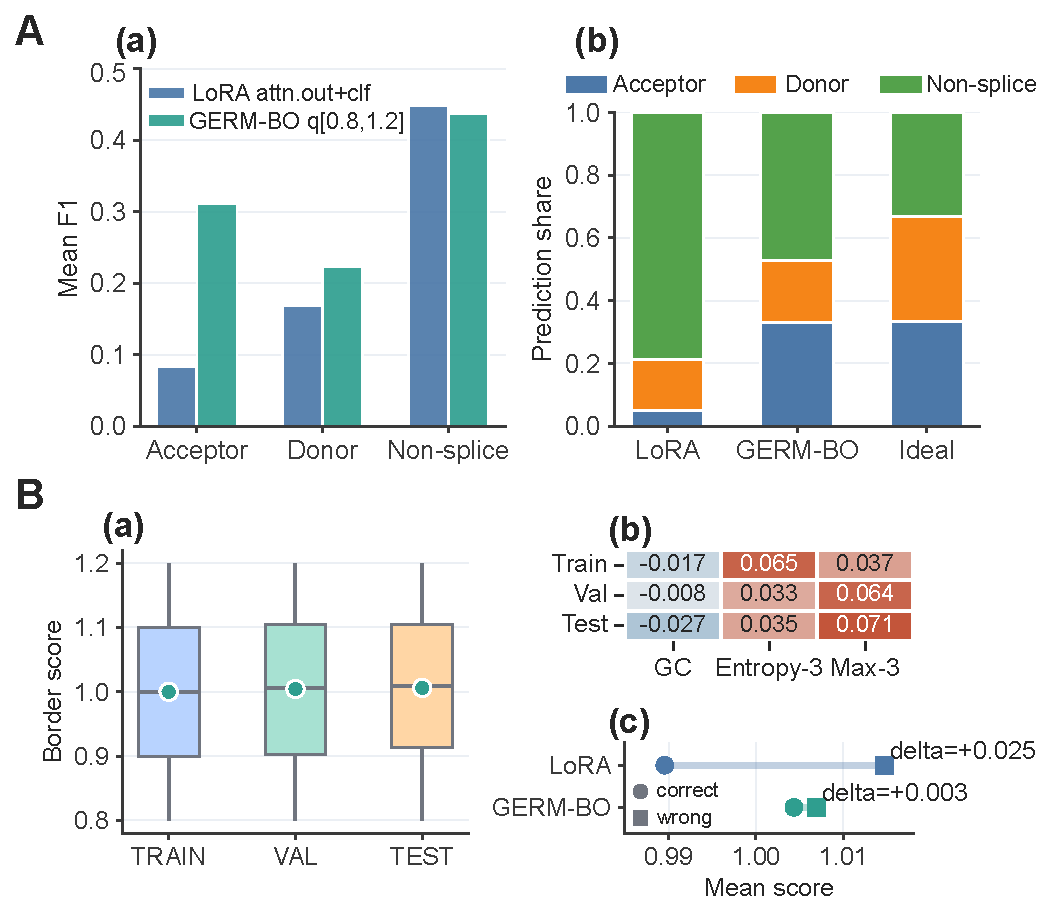
\includegraphics[width=0.95\linewidth]{figs/0910.pdf}
\caption{Class recovery and estimator quality on the strict splice split (Supplementary Fig.~S2).}
\label{fig:why_it_works}
\end{figure}

\begin{figure}[htbp]
\centering
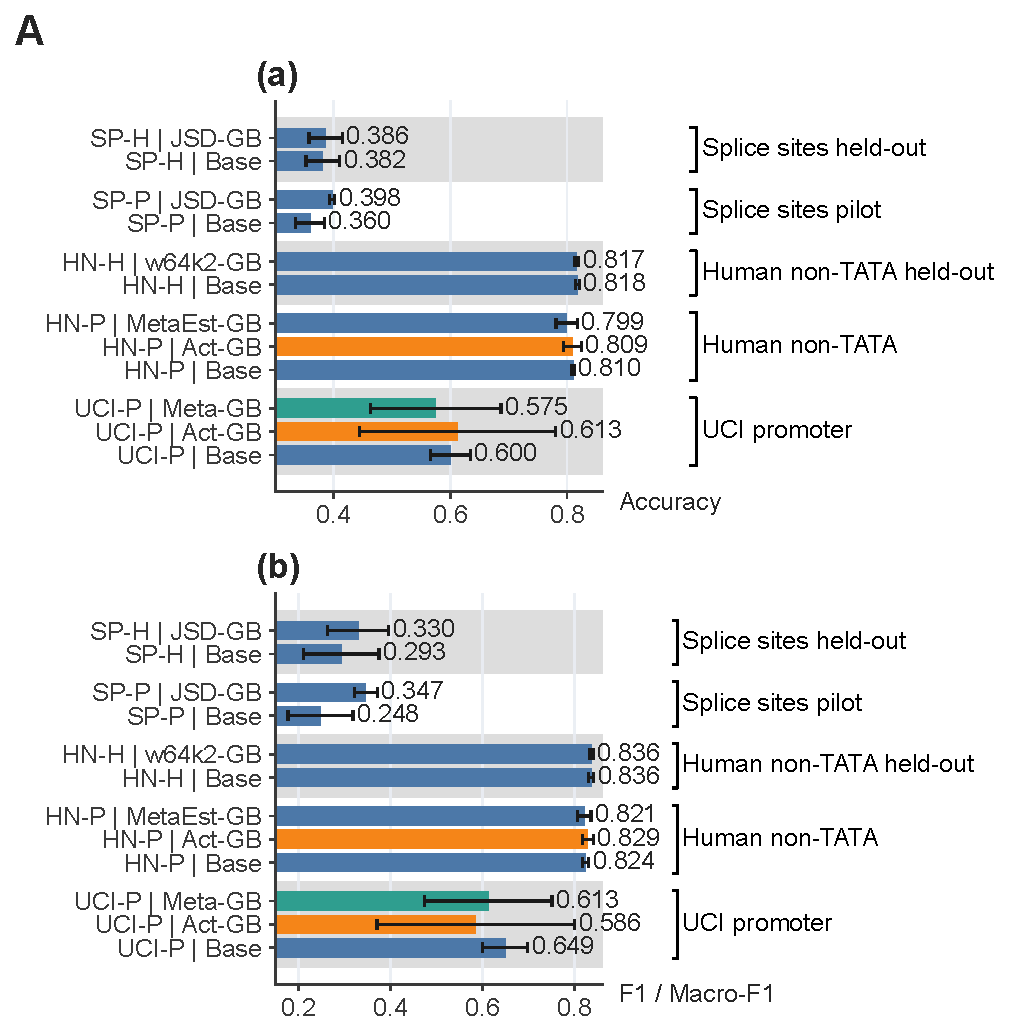
\includegraphics[width=0.95\linewidth]{figs/05_external_benchmark_overview.pdf}
\caption{External pilot overview across promoter and splice datasets (Supplementary Fig.~S1).}
\label{fig:external_benchmark_overview}
\end{figure}

\subsection{Promoter and chromatin null/near-null regimes}

On Genomic Benchmarks \splitname{human\_nontata\_promoters} (held-out seeds 45--49), LoRA reaches $0.8178 \pm 0.0034$ accuracy and label-free GERM-BO reaches $0.8168 \pm 0.0032$ ($\Delta=-0.0010$).

DNABERT-2 histone and enhancer pilots (pilot seeds 42--44; held-out 45--49) do not establish a robust label-free advantage: no held-out task has a bootstrap CI excluding zero, and pilot/held-out sign agreement is limited. NT v2 50M histone pilots similarly show positive mean deltas on only three of ten marks. Label-free strict-splice transfer is robust on DNABERT-2 but inconclusive on NT v2 50M and near-null on HyenaDNA tiny (main text Discussion).

\subsection{Sensitivity and resource footprint}

On held-out controlled splits, $\lambda_{\mathrm{comp}}\in\{0.15,0.20,0.25,0.27\}$ is stable; $\lambda_{\mathrm{comp}}=0.27$ is near-optimal on \splitname{border\_hard}. Rank $r\in\{4,8,16\}$ remains competitive at the default $r=8$. On the strict splice setting (seed 50), GERM-BO and LoRA share the same trainable parameter count ($30{,}744$) and peak memory ($587$\,MB); end-to-end times are comparable because compensation is elementwise scaling on the LoRA branch.

\end{document}
